% !TeX program = latexmk
% !TeX spellcheck = pl_PL
% !TeX root = example.tex

\chapter{Architektura aplikacji}

Projekt aplikacji wspomagającej zdalne szacowanie historyjek metodą Planning Poker
został wykonany w technologii, która pozwala na korzystanie z niej przy pomocy przeglądarki internetowej.

Architektura aplikacji oparta została o dwa podstawowe narzędzia:
ReactJS po stronie \textit{frontendu} oraz Firebase po stronie \textit{backendu}.
ReactJS to biblioteka napisana w języku JavaScript, stworzona przez firmę Facebook,
dzięki której budowanie dużych oraz kompleksowych interfejsów użytkownika staje się łatwiejsze.

Firebase z kolei to usługa świadczona przez firmę Google, która
pozwala na trwałe przechowywanie danych w chmurze, oferując przy tym
wsparcie dla obustronnej komunikacji protokołem Websocket, wykorzystywanym często
przez aplikacje internetowe wymagające interakcji pomiędzy użytkownikami w czasie rzeczywistym.

\section{Czym jest ReactJS}

Twórcy ReactJS opisują go jako Widok (ang. View) w architekturze MVC.
Wprowadza bardzo wydajny sposób utrzymania widoku zsynchronizowanego ze stanem danych
przechowywanym w pamięci przeglądarki w postaci obiektu Javascript.

Ten specjalny stos który renderuje HTML używa wyjątkowo szybkiego algorytmu opartego na wirtualnym drzewie DOM,
które jest ``lżejszym'' odpowiednikiem drzewa DOM. ReactJS wykorzystuje je
do minimalizacji liczby zmian w rzeczywistym drzewie DOM, potrzebnych do wprowadzenia go
w stan bezpośrednio wynikający z kształtu powiązanych danych.

Efektem tego algorytmu jest bardzo duża wydajność aplikacji korzystających z ReactJS oraz
łatwość pisania tych aplikacji ze względu na to, iż większością optymalizacji związanych
z renderowanie interfejsu użytkownika zajmuje się wspomniany algorytm.

Ponadto ReactJS ma jednokierunkowy, reaktywny przepływ danych,
który jest znacznie bardziej zrozumiały i łatwiejszy w rozwoju od podejścia tradycyjnego,
czyli wielokierunkowej komunikacji pomiędzy komponentami.

Komponenty – podstawowe bloki aplikacji React'owych – są zorganizowane w drzewie hierarchicznym,
w którym komponenty-rodzice wysyłają dane do swoich dzieci przez zmienne właściwości.
Każdy komponent ma także zmienną stanu, która determinuje obecne dane dla tego widoku.
Za każdym razem, gdy stan jest zmieniany, komponent wywołuje metodę \textit{render},
a React znajduje najbardziej efektywną metodę aktualizacji drzewa DOM.

Odkąd głównym zadaniem React’a jest interfejs użytkownika,
aplikacje na nim zrobione potrzebują czegoś jeszcze,
co będzie zachowywało się jak tzw. \textit{backend}, czyli sposób na trwałe
przetrzymywanie danych, nieleżne od stanu przeglądarki, która służy jako
środowisko uruchomieniowe dla ReactJS.
Do tego celu zdecydowałem się na użycie usługi Firebase.
Firebase dostarcza model (ang. Model) i kontroler (ang. Controller) w MVC
do aplikacji napisanych w ReactJS, czyniąc z nich w pełni funkcjonalne aplikacje,
których stan nie zależy wyłącznie od przeglądarki internetowej, w której działają.
Używając React’owego jednokierunkowego systemu wiązania danych łatwo jest zintegrować go z Firebase.
\cite{www_react}

\section{Firebase}

Firebase jest platformą dla aplikacji webowych oraz mobilnych, która wprowadza
dla deweloperów mnóstwo narzędzi oraz usług pomagających im tworzyć wysokiej jakości
aplikacje oraz zwiększyć ich bazę użytkowników.

\subsection{Historia Firebase}

W 2011 roku Firebase znany był pod nazwą Envelope.
Jako Envelope wprowadził dla deweloperów API,
które umożliwiało wprowadzenie komunikatora do ich strony internetowej.

Interesującym było to, że ludzie używali aplikacji by przekazywać dane,
które były czymś więcej niż wiadomościami komunikatora.
Deweloperzy aplikacji internetowych (w tym gier) używali Envelope
w celu synchronizacji danych aplikacji jak i stanu gry
w czasie rzeczywistym pomiędzy ich użytkownikami.

To doprowadziło założycieli Envelope, Jamesa Tamplina oraz Andrew Lee
do pomysłu by rozdzielić komunikator online oraz platformę wymiany danych w czasie rzeczywistym.
W kwietniu 2012 Firebase powstał jako oddzielna firma które wprowadziła usługę backendu
(ang. BaaS, Backend-as-a-Service) z funkcjonalnościami czasu rzeczywistego.

Po tym jak firma została przejęta przez Google w 2014 roku,
szybko ewoluowała do wielofunkcyjnej platformy mobilnej oraz webowej jaką znamy dzisiaj.

\section{Usługi Firebase wykorzystane w pracy}

% Rysunek
\begin{figure}
	\centering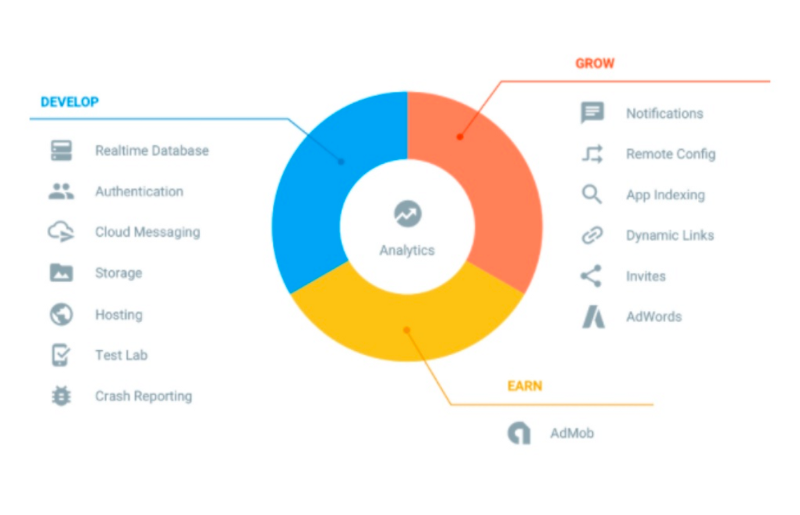
\includegraphics[width=.6\textwidth]{img/firebase}
	\caption{Usługi Firebase.[hackernoon.com]}\label{rys:firebase}% Źródło rysunku i etykieta przez którą odwołujemy się do rysunku.
\end{figure}

\subsection{Firebase Authentication}

W swojej aplikacji przede wszystkim skorzystałem z usługi \textit{FireBase Authentication},
która wprowadza usługi serwerowe,
łatwe narzędzia dla deweloperów oraz biblioteki Javascript
znacząco przyspieszające implementację oraz bezpieczeństwo
funkcji związanych z rejestracją oraz uwierzytelnieniem w aplikacji.

Autor skorzystał z usług logowania anonimowego oraz
tzw. \textit{third-party authentication} w usłudze Github, poprzez protokół OAuth.
Uwierzytelnienie poprzez usługę Github pozwala na integrację aplikacji z
narzędziem Github, co jest funkcją kluczową dla realizacji celu projektu.

\subsection{Firestore}

Firestore jest nierelacyjną bazą dokumentów, która pozwala łatwo przechowywać,
synchronizować oraz przeszukiwać dane w aplikacjach mobilnych oraz webowych – w globalnej skali.

Firestore przechowuje dane w postaci obiektów zwanych dokumentami.
Te dokumenty posiadają pary klucz-wartosć oraz mogą zawierać jakiekolwiek rodzaje danych
od łańcuchów po dane binarne a nawet obiekty, które przypominają format JSON.
Dokumenty są pogrupowane w kolekcje.
\ref{rys:firestoreData}

\begin{figure}
	\centering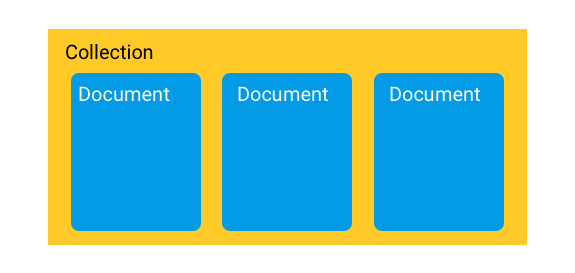
\includegraphics[width=.6\textwidth]{img/firestoreData}
	\caption{Postać danych w firestore [hackernoon.com]}\label{rys:firestoreData}% Źródło rysunku i etykieta przez którą odwołujemy się do rysunku.
\end{figure}

Fierstore może zawierać wiele kolekcji zawierających dokumenty, które wskazują na subkolekcje.
Te subkolekcje mogą znowu zawierać dokumenty oraz swoje subkolekcje i tak dalej.
Można zatem powiedzieć że jest to hierarchiczny model danych (patrz \ref{rys:firestoreTree}).
\cite{www_hakermoon}

\begin{figure}
	\centering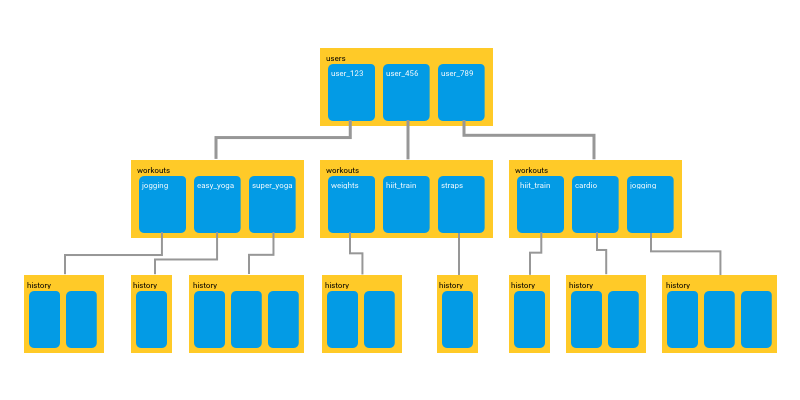
\includegraphics[width=.6\textwidth]{img/firestoreTree}
	\caption{Ułożenie danych w firestore [hackernoon.com]}\label{rys:firestoreTree}% Źródło rysunku i etykieta przez którą odwołujemy się do rysunku.
\end{figure}

\section{Redux czyli implementacja architektury Flux}

Jedną z najważniejszych cech komponentów ReactJS jest wbudowany w nie stan.
Jest to bardzo przydatna koncepcja. Komponent posiada stan,
który może ulec zmianie w wyniku interakcji użytkownika z aplikacją.
Zmiana stanu pociąga za sobą operację re-renderowania drzewa Virtual DOM.
W wyniku tego, pewne części interfejsu widocznego na ekranie ulegają zmianie.
Oczywiście wiadomym jest też, że jeden komponent może zależeć od innego komponentu.
Możemy przecież przekazywać stan komponentu rodzica do jego komponentów dzieci itd.

To wszystko działa świetnie. Niestety w miarę jak aplikacja rośnie,
rozrasta się poziom skomplikowania poszczególnych komponentów.
Z tego względu programiści Facebooka, odpowiedzialni za rozwój ReactJS, wymyślili
architekturę aplikacji, która rozwiązuje ten problem.
Architektura ta nazwa się \textbf{Flux}.
\cite{www_nafrontendzie}

\subsection{Architektura FLUX}

Flux jest architekturą, której Facebook używa do budowania aplikacji po stronie klienta.
Jest to uzupełnienie komponentów React’a przez wykorzystanie jednokierunkowego przepływu danych.
Nie jest to gotowe narzędzie, czy biblioteka, lecz pewien wzorzec architektoniczny.
Można z niego korzystać bez wielu nowych linijek kodu.

\begin{figure}
	\centering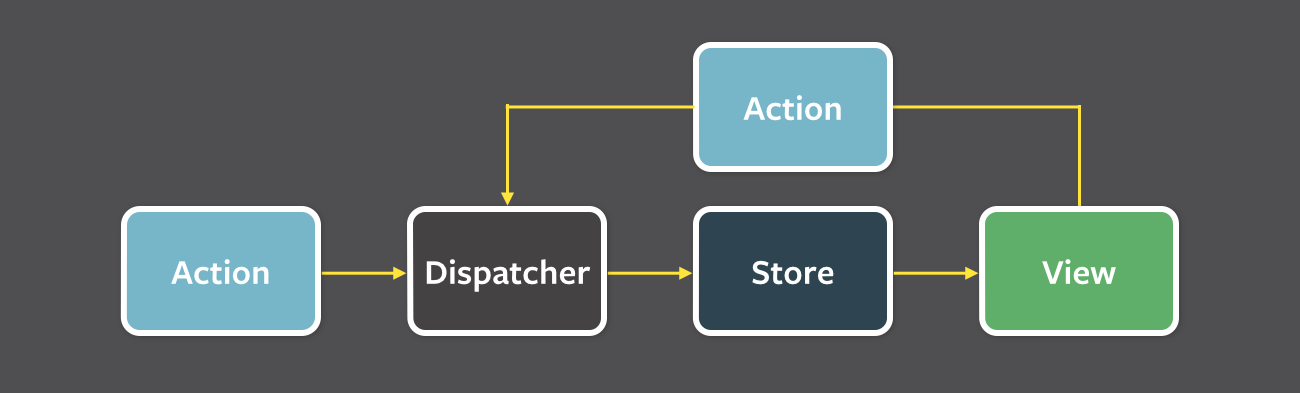
\includegraphics[width=.6\textwidth]{img/flux}
	\caption{Architektura Flux [wwww.nafrontendzie.pl]}\label{rys:flux}% Źródło rysunku i etykieta przez którą odwołujemy się do rysunku.
\end{figure}

Przepływ rozpoczyna się od lewej strony.
Najpierw tworzone jest akcja – jest to zwykły obiekt zawierający właściwość \texttt{type}.
Oprócz tego może on posiadać więcej właściwości służących do przekazywania dodatkowych danych.
Akcja taka tworzona jest przez funkcję zwaną \textit{action creator}, czyli kreator akcji.
W przypadku Redux, akcja jest zwykłą funkcją.

% lub {java} albo {bash} albo {text}
\begin{listing}
\begin{minted}{c}
const mapStateToProps = (state) => {
    return { counter: state.counter };
};
const mapDispatchToProps = (dispatch) => {
    return {
        onIncrement: () => dispatch({ type: 'INCREMENT' }),
        onDecrement: () => dispatch({ type: 'DECREMENT' })
    }
};

Counter = connect(mapStateToProps, mapDispatchToProps)(Counter);
\end{minted}
\caption{Przykładowe akcje licznika i ich stan} \label{listing:licznik}
\end{listing}

W listingu \ref{listing:licznik} przedstawiony jest prosty licznik z dwoma akcjami,
które zwiększają bądź zmniejszają licznik o jeden.
Stan oraz funkcje rozsyłające dostępne są w obiekcie \texttt{this.props}.
Spójrzmy na kod odpowiedzialny za ich mapowanie.
\begin{center}
	\textbf{Funkcja mapStateToProps}
\end{center}
Funkcja \texttt{mapStateToProps} pobiera \texttt{state} jako parametr i zwraca nowy obiekt.
Częstą praktyką jest po prostu przekazanie całego stanu do właściwości,
jednak jest to też właściwe miejsce by odfiltrować dane.
\begin{center}
	\textbf{Funkcja mapDispatchToProps}
\end{center}
Kolejna funkcja to \texttt{mapDispatchToProps}. Zwraca ona obiekt zawierający metody.
Za pomocą wywołania funkcji \texttt{dispatch} rozgłasza ona obiekty akcji do \texttt{store}.
Metoda \texttt{dispatch} przekazuje obiekty akcji bezpośrednio.

Zwykle w projekcie definiuje się to jako specjalne kreatory akcji.
Dzięki kreatorom możemy opóźnić wywołanie akcji lub zmienić dane w naszym Redux tylko wtedy,
gdy są spełnione określone warunki (patrz \ref{listing:firebase_action}).

% lub {java} albo {bash} albo {text}
\begin{listing}
\begin{minted}{c}
export const startAddUserToGame = (owner, repo, game, user = {}) => {
    return dispatch => {
        var userUpdate = {}

        const tempUser = {
            email: user.email,
            isAnonymous: user.isAnonymous,
            id: user.uid,
            name: user.displayName,
            online: true
        };

        userUpdate[`users.` + user.uid.toString()] = tempUser
        const gameRef = db
        .collection(`users`)
        .doc(owner.toString())
        .collection(`repos`)
        .doc(repo.toString())
        .collection(`games`)
        .doc(game.toString())

        gameRef.update(userUpdate).then(() => {
            dispatch(addUserToGame(owner, repo, game, tempUser))
        });
    }
}
\end{minted}
\caption{Przykładowy kreator akcji z projektu} \label{listing:firebase_action}
\end{listing}

W tym przykładzie gracz jest dodawany do gry tylko wtedy,
gdy jest uczestnikiem gry w bazie danych Firestore.
Jak widać w przykładzie, kreator zwraca funkcję,
która wykorzystuje \texttt{dispatch} by wysłać akcję do store.
Aby zadziałać, funkcja musi znać dokładną lokalizację gry w bazie oraz dane użytkownika.
Aby dostać się do gry, musimy znać właściciela oraz nazwę repozytorium w której znajduje się gra
oraz identyfikator gry.

Dzięki funkcji \texttt{update} gracz jest dodawany do gry dostając się odpowiednio do obiektu \texttt{users},
dokumentu gry, kolekcji repozytoria, dokumentu naszego repozytorium.
Kolekcja gier znajduje się w repozytorium, a dzięki znajomości identyfikatora gry
dostajemy się do jej obiektu i wstawiamy do niej obiekt gracza.
Jeżeli akcja w bazie danych zakończy się sukcesem, rozsyłamy akcję dodawania gracza do store.

\begin{center}
	\textbf{Funkcja connect}
\end{center}
Wracając do mapowania. W przedstawionym wcześniej przykładzie najbardziej istotna jest ostatnia jego linia.
Wywołuję ona funkcję \texttt{connect}.
Przyjmuje ona funkcje \texttt{mapStateToProps} oraz \texttt{mapDispatchToProps}
jako parametry i wyniki ich wywołania łączy w odpowiedni obiekt.
Następnie zwraca funkcję, która jako parametr przyjmuje komponent.
Funkcja ta wprowadza przygotowany wcześniej obiekt do \texttt{this.props} tego komponentu.

Funkcja connect opakowuje przekazany komponent i zwraca nową jego wersję.

Wracając do Flux. Tak tworzona akcja jest dostarczana do store za pomocą wywołania funkcji \texttt{dispatcher}.
Funkcja ta w zasadzie zarządza całym przepływem danych.
Każdy store w aplikacji rejestruje w dispatcherze swoje funkcje wywołania zwrotnego
w celu obsługi przychodzących akcji.
W momencie gdy akcja jest rozsyłana (ang. dispatch), wywoływane są po kolei wszystkie
funkcje wywołania zwrotnego (ang. callback).
Jeden z nich powinien umieć rozpoznać akcję po jej typie i być przygotowany na jej odpowiednią obsługę.

\begin{center}
	\textbf{Funkcja reducer}
\end{center}

W przypadku Redux'a rolę store'a pełni funkcja \textit{reducer}. Dzięki temu, że jest to funkcja,
można ją jednocześnie użyć jako funkcję wywołania zwrotnego,
którą store uruchomi w momencie gdy zostanie rozgłoszona jakaś akcja.
Funkcja ta przyjmuje dwa parametry: \texttt{state} oraz \texttt{action}.

Działa to tak: ktoś wywołuje akcję, obiekt \textbf{store} wywołuje funkcję \textbf{reducer},
przekazując do niej aktualny stan oraz akcję, \textbf{reducer}
sprawdza typ przekazanej do niej akcji i w zależności od tego jaki jest ten typ,
zwraca nową wersję obiektu stanu (patrz przykład \ref{listing:reducer}).

\begin{listing}
\begin{minted}{c}
const reducer = (state, action) => {
    switch (action.type) {
        case 'INCREMENT':
            return { ...state, counter: state.counter + 1 };
        case 'DECREMENT':
            return { ...state, counter: state.counter - 1 };
        default:
            return state;
    }
};
\end{minted}
\caption{Przykładowy reducer licznika} \label{listing:reducer}
\end{listing}

W przykładzie, jeśli typ akcji to `INCREMENT' to zwracany jest nowy obiekt stanu,
który ma zwiększoną o jeden wartość atrybutu \texttt{counter}.
Jeśli natomiast typ akcji to `DECREMENT' to zwracany jest nowy stan z atrybutem
\texttt{counter} zmniejszonym o jeden.
Jeśli typ akcji jest w tym miejscu nieznany, wykonujemy domyślną (ang. default) operację, którą jest
przekazanie obiekt stanu w niezmienionej postaci.

Generalnie wszystkie obiekty store zawierają łącznie cały stan aplikacji.
Store zawiera implementację funkcji wywoływania zwrotnego,
która jest rejestrowana w ``dispatcherze'', i która obsługuje akcje związane z danym store.
Cechą Reduxa jest to, że cały stan jest przechowywany w jednym obiekcie.

Kolejny element na diagramie to widok.
Można powiedzieć, że jest on reprezentowany po prostu przez komponent ReactJS.
Używa on stanu aplikacji zapisanego w obiekcie store, tak jakby był on wewnętrznym stanem komponentu.
Zmiana stanu w store powoduje re-renderownie komponentu.
Dodatkowo komponent widoku może rozsyłać kolejne akcje, na przykład kiedy użytkownik
kliknie na jakiś przycisk interfejsu na ekranie.
To powoduje zmianę stanu zapisanego w store.
W Redux komponent ma dostęp do akcji i stanu dzięki wspomnianej przeze mnie wcześniej funckji \texttt{connect}.

Wszystko to po prostu zestaw zasad.
To programista może zdecydować jak to dokładnie będzie zaimplementowane.
Na szczęście nie jest on zdany sam na siebie, ponieważ istnieje kilka gotowych
implementacji architektury Flux w postaci bibliotek.
Jedną z nich jest oczywiście Redux.
\cite{www_nafrontendzie}

\subsection{Czym Redux różni się od Flux}

Redux jest inspirowany pewnymi ważnymi cechami architektury Flux.
Tak jak Flux, Redux przepisuje model danych do oddzielnej warstwy aplikacji
(\textit{stores} w Flux, \textit{reducers} w Redux).

Tak jak we Flux, wszystkie operacje na danych są opisywane w postaci akcji.
W przeciwieństwie do Flux, Redux jednak nie ma konceptu rozsyłacza,
ponieważ opiera się na czystych funkcjach zamiast obiektów emiterów akcji,
a czyste funkcje są łatwe do tworzenia i nie potrzebują żadnej encji
(reprezentacja wyobrażonego lub rzeczywistego obiektu) by nimi zarządzać.
Jest to więc pewne odstępstwo od Flux’a.
\cite{www_nafrontendzie}

Inną ważną różnicą od Flux jest to, że Redux zakłada niemutowalność danych.
Możesz używać statycznych obiektów oraz tablic dla swojego stanu,
ale mutowanie ich wewnątrz reducerów jest bardzo odradzane,
dlatego po zmianie stanu zawsze powinien być zwracany nowy obiekt (patrz rysunek \ref{rys:reduxFlux}).

Ogólnie Redux może być opisany przez trzy fundamentalne zasady:
\begin{itemize}
	\item Pojedyncze źródło prawdy: stan całej aplikacji przetrzymywany jest
	w drzewie obiektów wewnątrz pojedynczego obiektu store.
	\item Stan jest tylko do odczytu: jedynym sposobem na zmianę stanu jest wywołanie akcji,
	która zwraca obiekt opisujący co powinno się stać.
	\item Zmiany wykonywane są w ramach czystych funkcji: aby określić jak drzewo stanu
	transformowane jest przez akcje, musisz tworzyć ``czyste reducery''.
\end{itemize}

\begin{figure}
	\centering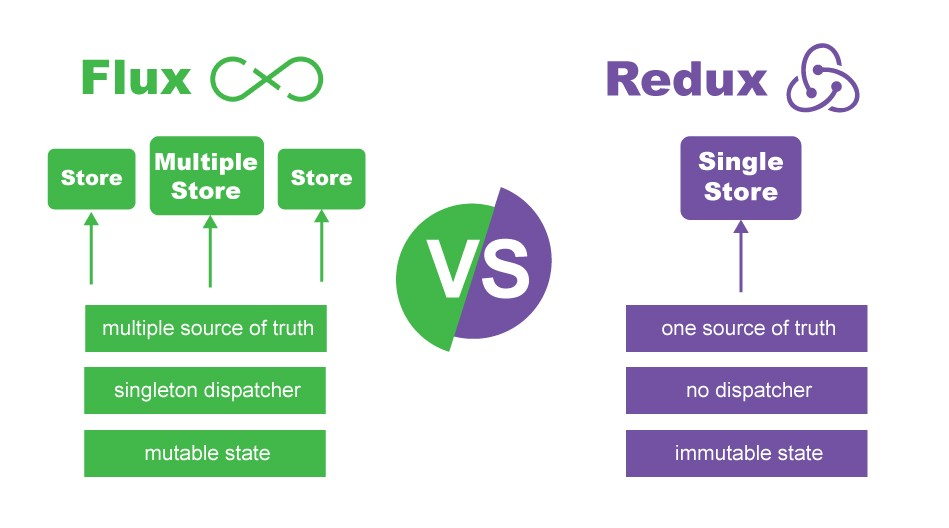
\includegraphics[width=.6\textwidth]{img/reduxFlux}
	\caption{Różnice między Redux a Flux [www.medium.com]}\label{rys:reduxFlux}% Źródło rysunku i etykieta przez którą odwołujemy się do rysunku.
\end{figure}

\subsection{redux-thunk}

Biblioteka \textbf{redux-thunk} została stworzona przez Dana Abramova,
który jednocześnie jest twórcą Reduxa. Pozwala ona tworzyć kreatory akcji,
które zamiast obiektu zwracają funkcję.
Dzięki temu możliwe jest opóźnienie rozgłoszenia akcji lub zgłoszenie jej tylko
jeśli zostaną spełnione określone warunki. \cite{www_thunk}

Jak dodać thunk do Reduxa pokazuje listing \ref{listing:thunk-redux}.

\begin{listing}
\begin{minted}{c}
    import { createStore, applyMiddleware } from 'redux';
    import thunk from 'redux-thunk';
    import rootReducer from './reducers/index';

    const store = createStore(
        rootReducer,
        applyMiddleware(thunk)
    );
\end{minted}
\caption{Połączenie Reduxa i Thunka} \label{listing:thunk-redux}
\end{listing}

\begin{center}
	\textbf{Obsługa wywołań asynchronicznych czyli kreatory akcji}
\end{center}

W przykładzie (listing \ref{listing:firebase_action}) widnieje akcja,
która najpierw dodaje użytkownika do bazy, a następnie rozgłasza akcję dodawania użytkownika,
jeżeli modyfikacja danych w bazie zakończyła się pomyślnie.

W funkcji \texttt{startAddUserToGame} pobierane są najpierw dane o grze, czyli: \texttt{owner},
który jest po prostu identyfikatorem użytkownika Githuba.
Następnie jest pobierany identyfikatory gry \texttt{game}.
Na końcu dostajemy dane użytkownika, którego chcemy dodać do gry.

Funkcja ta zwraca funkcję przyjmującą parametr \texttt{dispatch},
który służy do rozgłaszania danych.
Później jest tworzony użytkownik, który ma zostać dodany do gry (\texttt{tempUser}).
Na końcu jest tworzony obiekt, będący odnośnikiem do użytkowników w bazie,
który pomaga zaktualizować obiekt gry.
Finalnie korzystając z referencji aktualizuje się obiekt gry w bazie danych,
a w razie sukcesu (funkcja \textbf{then}) akcja jest rozsyłana dalej.

\subsection{Połączenie Firebase i Redux}

Jak nie trudno się domyślić, wszystkie operacje pomiędzy Firebase a Redux są realizowane w postaci akcji.
Do synchronizacji frontend i backend służy \textit{Thunk},
który przesyła dane do store’a tylko wtedy,
kiedy nie ma żadnych problemów po stronie Firebase.

Jeżeli baza danych nie będzie mogła pobrać danych bo wystąpił błąd,
Thunk nie wykona żadnych operacji. Sposób połączenia tych dwóch elementów przedstawiono
na rysunku \ref{rys:fireRedux}.

\begin{figure}
	\centering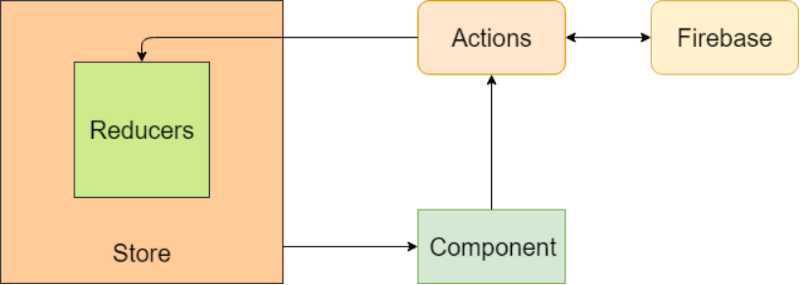
\includegraphics[width=.6\textwidth]{img/fireRedux}
	\caption{Sposób połączenia firebase i reduxa. [medium.com]}\label{rys:fireRedux}% Źródło rysunku i etykieta przez którą odwołujemy się do rysunku.
\end{figure}
